\chapter{Release 2 --- Project and Operational Management}

\section*{Introduction}
Release~1 delivered a secured and administrable platform, but one that managed no project. This
release opens operational steering. Sprint~3 introduces the central entity of the whole domain ---
the project, with its controlled lifecycle and its budget; Sprint~4 populates it with a team and
with the workload data on which every later indicator depends.

At the end of this release, a project can be created, staffed, planned, and its actual consumption
recorded: everything the financial engine of Release~3 will need as input.

% =====================================================================
\section{Sprint 3 --- Project Management and Lifecycle}

\subsection{Sprint Objective}
Deliver the management of projects: creation with their contractual and financial identity,
assignment of a project manager, and a lifecycle that the application enforces rather than merely
documents.

\subsection{Functional Scope}
This sprint covers user stories US-08 to US-10: creating and configuring a project, controlling its
status transitions, and assigning its project manager.

\subsection{Features Implemented}
\begin{itemize}
  \item Project creation with code, client, funder, engagement type, currency and budget.
  \item Controlled status lifecycle with server-side enforcement.
  \item Effective budget derived from the initial budget and its amendments.
  \item Project manager assignment, with a single active assignment at a time.
  \item Project archiving, distinct from closure.
\end{itemize}

\subsection{Technical Realisation}

\subsubsection{Project identity}
The \texttt{project} module reproduces the identification sheet of the reference workbook: project
code, client, funder, business model, engagement type (fixed price or time~\&~material), project
currency with its contractual exchange rate, initial budget, sold workload and provisions. The
class model of the module is given in Figure~\ref{fig:class-proj}.

\begin{figure}[H]
  \centering
  
\includegraphics[width=0.85\columnwidth]{img/class_project_team.png}
  \caption{Class diagram --- projects and teams}
  \label{fig:class-proj}
\end{figure}

\subsubsection{A lifecycle enforced by the domain}
A project moves through five states: \texttt{DRAFT}, \texttt{ACTIVE}, \texttt{ON\_HOLD},
\texttt{COMPLETED} and \texttt{CANCELLED}. Not every transition is legal: a completed project
cannot return to draft, a cancelled project is terminal.

The rule is carried by the enumeration itself, through a \texttt{canTransitionTo} operation that
each status answers for its own legal successors. The service layer consults it before any status
change and rejects an illegal transition with \texttt{HTTP 422 Unprocessable Entity}. Placing the
rule in the domain rather than in the controller guarantees that no future entry point can bypass
it.

\begin{figure}[H]
  \centering
  
\includegraphics[width=0.7\columnwidth]{img/state_project.png}
  \caption{State diagram --- project lifecycle}
  \label{fig:state}
\end{figure}

Archiving is deliberately \textbf{not} a state but a flag on a completed project: an archived
project leaves the active lists while remaining restorable, which a terminal state would not allow.

\subsubsection{Effective budget}
A project carries an initial budget and, once amendments exist, a revised budget. Every computation
uses the \textbf{effective budget}: the revised budget when it is defined, the initial budget
otherwise. This value has a \textbf{single writer}, the amendment, which prevents the two
figures from drifting apart, a failure mode observed in the original workbook where the budget was
edited in several places.

\subsubsection{Project manager assignment}
A project has exactly one active project manager at any time, but keeps the history of previous
assignments. Assigning a new manager therefore closes the current assignment rather than
overwriting it, preserving the traceability required for auditing.

% TODO: capture as img/ui_projects.png and img/ui_project_detail.png, then uncomment.
% \begin{figure}[H]
%   \centering
%   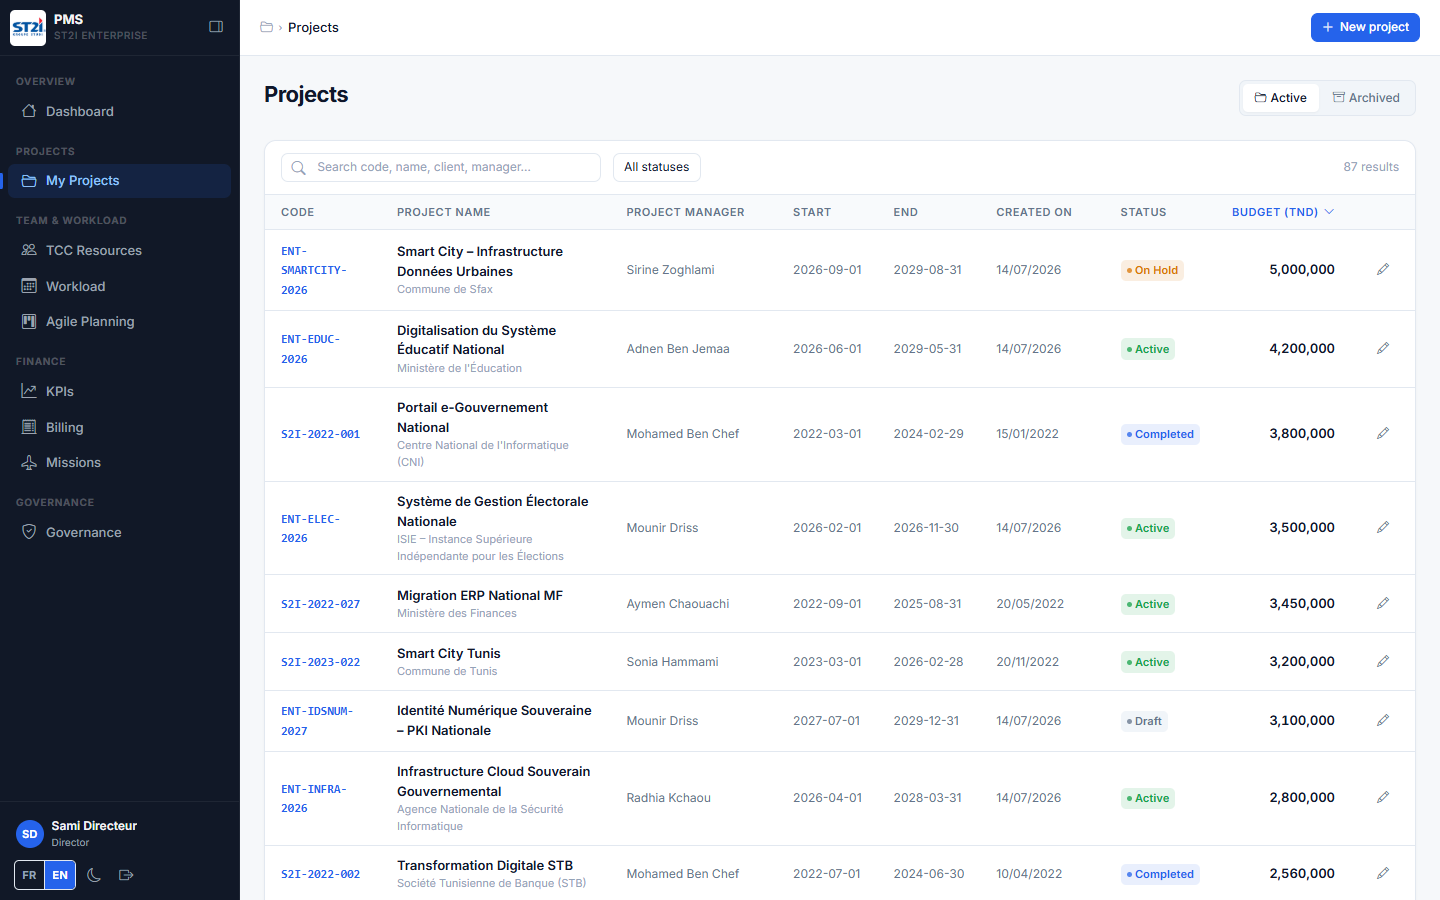
\includegraphics[width=0.95\columnwidth]{img/ui_projects.png}
%   \caption{Project list interface}
%   \label{fig:ui-projects}
% \end{figure}

\subsection{Tests and Validation}
Validation focuses on the lifecycle, since it is the rule most likely to be violated by a client
application.

\begin{longtable}{|m{4.2cm}|m{5.4cm}|m{4.8cm}|}
\hline
\textbf{Test case} & \textbf{Steps} & \textbf{Expected result} \\
\hline
\endhead
\endfoot
\endlastfoot
\hline
Legal transition & Move a project from \texttt{DRAFT} to \texttt{ACTIVE} & HTTP 200, status updated
\\
\hline
Illegal transition & Move a project from \texttt{COMPLETED} back to \texttt{DRAFT} & HTTP 422,
status unchanged \\
\hline
Terminal state & Attempt any transition out of \texttt{CANCELLED} & HTTP 422 \\
\hline
Effective budget & Add an amendment then read the project & Computations use the revised budget \\
\hline
Manager assignment & Assign a second project manager & Previous assignment closed, one active
manager remains \\
\hline
\caption{Test cases --- Sprint 3}
\label{tab:tests-s3}
\end{longtable}

\subsection{Sprint Outcome}
Projects exist, carry their contractual and financial identity, and follow a lifecycle the
application enforces. The invalid states that a spreadsheet cannot prevent are now structurally
impossible.

\subsection{Transition to the Next Sprint}
A project without a team consumes nothing and produces no indicator. Sprint~4 therefore staffs the
project and captures the effort planned and consumed, the raw material of the whole financial
model.

% =====================================================================
\section{Sprint 4 --- Teams and Workload Management}

\subsection{Sprint Objective}
Allow a project manager to build the project team, plan the monthly workload, and let developers
record the effort actually consumed, with the guarantees of integrity the indicators will depend
on.

\subsection{Functional Scope}
This sprint covers user stories US-11 to US-14: building the team, planning the workload,
submitting actual workload, and validating it.

\subsection{Features Implemented}
\begin{itemize}
  \item Assignment and removal of team members, with preserved history.
  \item Monthly workload planning per resource.
  \item Submission of actual workload, restricted to assigned projects.
  \item Validation of submitted workload by the project manager.
  \item Immutability of a validated period.
\end{itemize}

\subsection{Technical Realisation}

\subsubsection{Team assignment}
A team assignment links a user to a project with a role in the team and a validity period. A
developer may belong to several projects simultaneously. Removing a member closes the assignment
rather than deleting it, so that past workload remains attributable.

Assignment is protected by \textbf{two distinct checks}, illustrated in
Figure~\ref{fig:seq-assign}: the caller must hold the \texttt{ASSIGN\_DEVELOPER} permission
\emph{and} the target project must fall within their scope. The permission answers ``what may I
do''; the scope answers ``on which projects''. Conflating the two would let a project manager act
on a project that is not theirs.

\begin{figure}[H]
  \centering
  
\includegraphics[width=0.95\columnwidth]{img/seq_assign_developer.png}
  \caption{Sequence --- assigning a developer, permission and scope}
  \label{fig:seq-assign}
\end{figure}

\subsubsection{Two kinds of workload}
The model distinguishes the \textbf{workload plan} (what is forecast) from the \textbf{actual
workload} (what was consumed). Both are stored as a monthly time series, one row per project,
resource and month, rather than as a wide grid of month columns.

\subsubsection{Period normalisation and uniqueness}
A month is stored as the first day of that month. This normalisation is what makes uniqueness
enforceable: without it, two entries for the same month recorded on different days would coexist
silently. A unique partial index guarantees a single retained value per cell, and it is that value
which feeds the indicator engine.

\subsubsection{Validation and immutability}
A developer submits their own workload, on assigned projects only. The project manager then
validates it. Once a period is validated it becomes \textbf{immutable}: a later correction cannot
silently rewrite a month on which a monthly review has already been based. This constraint is the
direct answer to the traceability weakness identified in the Excel process.

% TODO: capture as img/ui_workload.png, then uncomment.
% \begin{figure}[H]
%   \centering
%   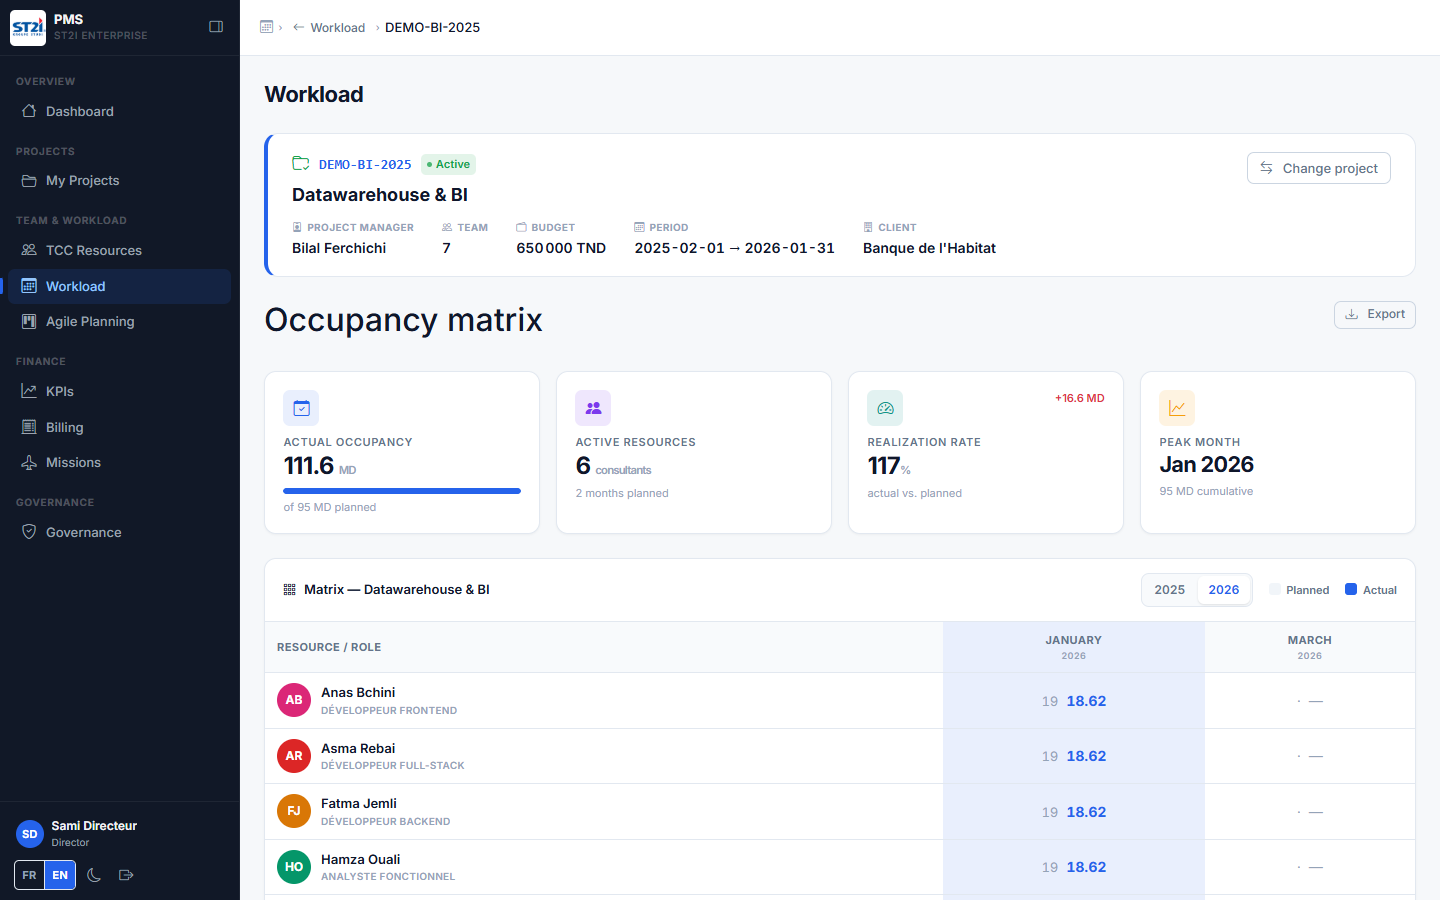
\includegraphics[width=0.95\columnwidth]{img/ui_workload.png}
%   \caption{Workload matrix interface}
%   \label{fig:ui-workload}
% \end{figure}

\subsection{Tests and Validation}

\begin{longtable}{|m{4.2cm}|m{5.4cm}|m{4.8cm}|}
\hline
\textbf{Test case} & \textbf{Steps} & \textbf{Expected result} \\
\hline
\endhead
\endfoot
\endlastfoot
\hline
Authorised assignment & Assign a developer with the permission, on a project in scope & HTTP 201,
assignment recorded \\
\hline
Out-of-scope assignment & Assign on a project outside the caller's scope & HTTP 403 \\
\hline
Submission on an unassigned project & Submit workload on a project the developer is not assigned to
& Refused \\
\hline
Duplicate month & Submit twice for the same project, resource and month & A single retained value
\\
\hline
Validated period & Modify a period already validated & Refused, period immutable \\
\hline
\caption{Test cases --- Sprint 4}
\label{tab:tests-s4}
\end{longtable}

\subsection{Sprint Outcome}
Projects now carry a team, a forecast and a measured consumption, all captured under integrity
constraints that a spreadsheet cannot express: no duplicate month, no entry on an unassigned
project, no silent rewriting of a validated period.

\subsection{Transition to the Next Sprint}
The cost side of the project is now measurable. The revenue side is not: nothing yet records what
is invoiced, nor the expenses that weigh on the margin. Release~3 delivers the financial and
governance value of the platform, starting with billing and missions.

\section*{Conclusion}
Release~2 turned a secured shell into an operational tool: projects with an enforced lifecycle,
teams with traceable assignments, and workload captured as a reliable monthly time series. The data
required by the financial engine is now available and trustworthy, which is the precondition for
the indicators built in the next release.
